\section{Formalism}

\subsection{subsection one}

Some content on section two, subsection one. Follow by an equation:
\begin{equation}\label{eq:e1}
\mathcal{L}_{\rm SM}=\mathcal{L}_{\rm QCD}+\mathcal{L}_{\rm QED}+\mathcal{L}_{\rm Weak}+\mathcal{L}_{\rm Higgs}
\end{equation}

Some content describing the equation. Then another big equation:
\begin{eqnarray}
\mathcal{L}_{\rm QCD}
&=&\sum_f \bar{q}_{f,i}\left(i\slashed{\partial}\delta_{ij}+ig\slashed{A}_a\left(T_a^{(F)}\right)_{ij}-M_f\delta_{ij}\right)q_{f,j}\nonumber\\
&&-\frac{1}{2}{\rm tr}\left(F_{\mu\nu}F^{\mu\nu}\right)-\frac{\lambda}{2}\left(\eta\cdot A_a\right)^2\nonumber\\
&&+\eta_\mu\bar{c}_a\left(\partial^\mu\delta_{ad}-gC_{abd}A_b^\mu\right)c_d
\end{eqnarray}

Along with some description.
We can reference the first equation using this Eq. \ref{eq:e1}.
Some more content.

\subsection{subsection two}

We can insert a table using this:

\begin{table}[t]
\begin{center}
\def\arraystretch{2}
\begin{tabular}{c|c|C}
Channels		&	Diagrams		&	\bar{\sum}|\mathcal{M}|^2/g_s^4\\\hline
$qq'\rightarrow qq'$
& \raisebox{-0.45\height}{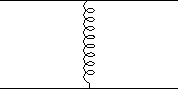
\includegraphics[height=1cm]{fig-feyns/qqqqt}}	
& \frac{4}{9}\frac{s^2+u^2}{t^2}\\
$qq\rightarrow qq$
& \raisebox{-0.45\height}{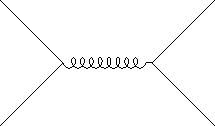
\includegraphics[height=1cm]{fig-feyns/qqqqs}~~~~~~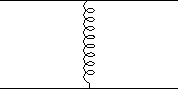
\includegraphics[height=1cm]{fig-feyns/qqqqt}} 
& \frac{4}{9}\left(\frac{s^2+u^2}{t^2}+\frac{s^2+t^2}{u^2}\right)-\frac{8}{27}\frac{s^2}{tu}\\
$q\bar{q}\rightarrow q'\bar{q}'$
& \raisebox{-0.45\height}{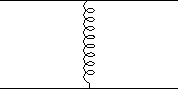
\includegraphics[height=1cm]{fig-feyns/qqqqt}} 
& \frac{4}{9}\frac{t^2+u^2}{s^2}\\
$q\bar{q}\rightarrow q\bar{q}$
& \raisebox{-0.45\height}{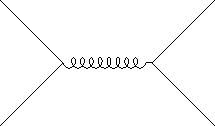
\includegraphics[height=1cm]{fig-feyns/qqqqs}~~~~~~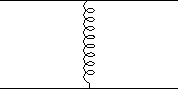
\includegraphics[height=1cm]{fig-feyns/qqqqt}} 
& \frac{4}{9}\left(\frac{s^2+u^2}{t^2}+\frac{t^2+u^2}{s^2}\right)-\frac{8}{27}\frac{u^2}{st}\\
$q\bar{q}\rightarrow gg$
& \raisebox{-0.45\height}{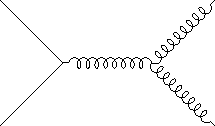
\includegraphics[height=1cm]{fig-feyns/qqggs}~~~~~~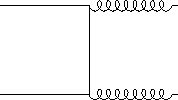
\includegraphics[height=1cm]{fig-feyns/qqggt}} 
& \frac{32}{27}\frac{t^2+u^2}{tu}-\frac{8}{3}\frac{t^2+u^2}{s^2}\\
$gg\rightarrow q\bar{q}$
& \raisebox{-0.45\height}{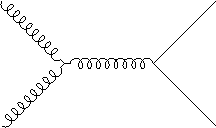
\includegraphics[height=1cm]{fig-feyns/ggqqs}~~~~~~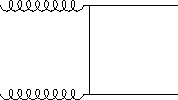
\includegraphics[height=1cm]{fig-feyns/ggqqt}} 
& \frac{1}{6}\frac{t^2+u^2}{tu}-\frac{3}{8}\frac{t^2+u^2}{s^2}\\
$gq\rightarrow gq$
& \raisebox{-0.45\height}{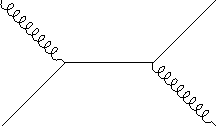
\includegraphics[height=1cm]{fig-feyns/gqgqs1}~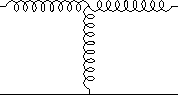
\includegraphics[height=1cm]{fig-feyns/gqgqt1}~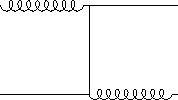
\includegraphics[height=1cm]{fig-feyns/gqgqt2}} 
& -\frac{4}{9}\frac{s^2+u^2}{su}+\frac{u^2+s^2}{t^2}\\
$gg\rightarrow gg$
& \raisebox{-0.45\height}{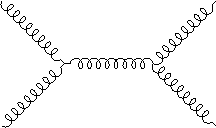
\includegraphics[height=1cm]{fig-feyns/ggggs1}~~~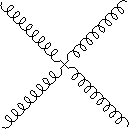
\includegraphics[height=1cm]{fig-feyns/ggggs2}~~~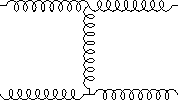
\includegraphics[height=1cm]{fig-feyns/ggggt}} 
& \frac{9}{2}\left(3-\frac{tu}{s^2}-\frac{su}{t^2}-\frac{st}{u^2}\right)
\end{tabular}
\end{center}
\caption{\label{tab:t1}Table caption.}
\end{table}

Add some description to the table, and reference it using Tab. \ref{tab:t1}.

\subsection{subsection three}

We can add reference to bibliography using this \cite{Hawking:1974rv},
or cite multiple references using this \cite{Hawking:1974rv,Antoniadis:2013pzd,Springel:2005nw}. Bibtex codes are stored in `main.bib' file.
Compile with pdflatex, then bibtex, then pdflatex again twice.

\pagebreak
